\chapter*{\FontH{\Huge Am Ufer des Dal Kar}}
\addcontentsline{toc}{chapter}{Am Ufer des Dal Kar}
\lettrine[lines=3]{\color{DeepPink}{M}}{}
\begin{sffamily}
mitten im Dschungel von Indien liegt der kleine See Dal Kar. Er hat die Form einer Ente. Beim Rücken und beim Kopf der Ente besteht das Ufer nur aus hohen Felsen. In den Felsen verstecken sich kleine Quellen, deren Wasser den See speisen. Viel Wasser kommt aber nicht an, das meiste verdunstet achon auf dem Weg nach unten als Nebel. Beim Bauch der Ente wird der See von undurchdringlichem Urwald überwuchert, der für grössere Tiere wie ein Zaun wirkt. Zugänglich ist der Dal kar nur auf Höhe der Füsse. Dal Kar gehört zu einem grossen Naturschutzgebiet, in dem auch der Wildhüter Amur arbeitet. Er hat mir folgende geschichte erzählt.
\end{sffamily}

Für Menschen ist der Dal Kar See fast unzugänglich. Er liegt weit entfernt vom nächsten Dorf und ausserdem ist es verboten, das Naturschutzgebiet zu betreten. Nur wir Wildhüter dürfen dort hin und glauben sie mir, das ist so aufregend wie anstrengend zugleich. Das Essen, das man mitnimmt, wird schon nach einem halben tag schimmelig, die Insekten versuchen ihr bestes, uns schnellstmöglich an jeder denkbaren Stelle des Körpers zu beissen und die schwüle Hitze ist anstrengend. Dafür wird man mit einer unglaublichen Natur belohnt. Es gibt alle Arten von Tieren hier, die man in Indien findet. Man sieht Pflanzen und Bäume, die es nur hier gibt und die manchmal noch nicht einmal einen Namen haben.

Meine Aufgabe am Dal Kar ist es aufzupassen, dass keine Wilderer kommen und im Auftrag der Universität Dehli die Tiere zu beobachten.

Der Dal Kar ist in einem grossen Gebiet der einzige See. Er ist wichtig für die meisten Tiere, den nauch sie müssen Baden, um gelegentlich das Ungeziefer aus dem Fell zu bekommen. Hirsche, Wildschweine, Muntjaks, Antilopen und noch viele andere Tiere kommen daher zu diesem See, um in ihm zu baden. Sie verlassen ihre Reviere und nehmen den weiten Weg auf sich.


Bei diesem See lebte aber ein riesiger Tiger, den grössten, den ich je gesehen habe. Wegen seiner Grösse habe ich ihn Shirkan getauft, so wie der Tiger aus dem Dschungelbuch. Shirkan war sehr schlau. Er hat sich einfach an der Stelle des Sees auf die Lauer gelegt, an dem alle Tiere, die baden wollten, vorbei mussten. 

War ein Tier so unvorsichtig, sich dem See zu nähern, war es schon verloren. Shirkan hat alle Tiere gerissen, ganz egal, ob er hungrig war oder nicht. Man konnte glauben, dass er den See für sich alleine haben wollte. Warum er so bösartig war, weiss ich nicht. Eigentlich ist es nicht die Art der Tiger, zu töten, wenn sie nicht hungrig sind oder zur Verteidigung. Shirkan hat das aber gemacht.

Das ist eine ganze Zeit so gegangen. Wäre es nicht ein Nationalpark, hätte ich tatsächlich überlegt, den zu schiessen. Aber es ist der wichtigste grundsatz für uns Wildhüter, nicht in die Natur einzugreifen. Die anderen Tiere haben sich mit der Zeit immer dichter rund um den See gedrängt, es sind immer mehr geworden. Viele waren wohl unschlüssig, was sie jetzt machen sollten. Ihre Reviere liegen oft weit entfernt und es dauert Wochen, bis sie wieder da sind.  Am schlimmsten war es wohl für die Büffel, für sie ist baden besonders wichtig.

Eines Tages gab es ein grosses Trompeten, denn eine Elephantenherde ist duch den park gezogen. Das kommt selten vor, denn im Dschungel sind Elephanten nur selten. Wahrscheinlich haben sie in ihren angestammten gebieten nicht mehr genug Futter gefunden. Die Menschen hier sind arm und versuchen alle Fläche für Felder zu nutzen, um das Überleben ihrer Familien zu sichern. Für die Elephanten ist das aber oft schlimm, denn dann fehlt ihnen genau dieser Platz.

Auch die Elephanten haben sich angezogen gefühlt von dem See und sind direkt auf ihn los marschiert. Zu meiner grossen Überraschung hat Shirkan sogar versucht, sie anzugreifen. Das ist natürlich selbst für den stärksten Tiger aussichtslos. Erst haben sich die Elephanten auch überhaupt nicht für sein Gebrüll interessiert. Für einen erwachsenen gesunden Epelphanten ist ja ein Tiger keine Bedrohung. 

\afterpage{
    \begin{figure}
        \thispagestyle{empty}
        \centering
        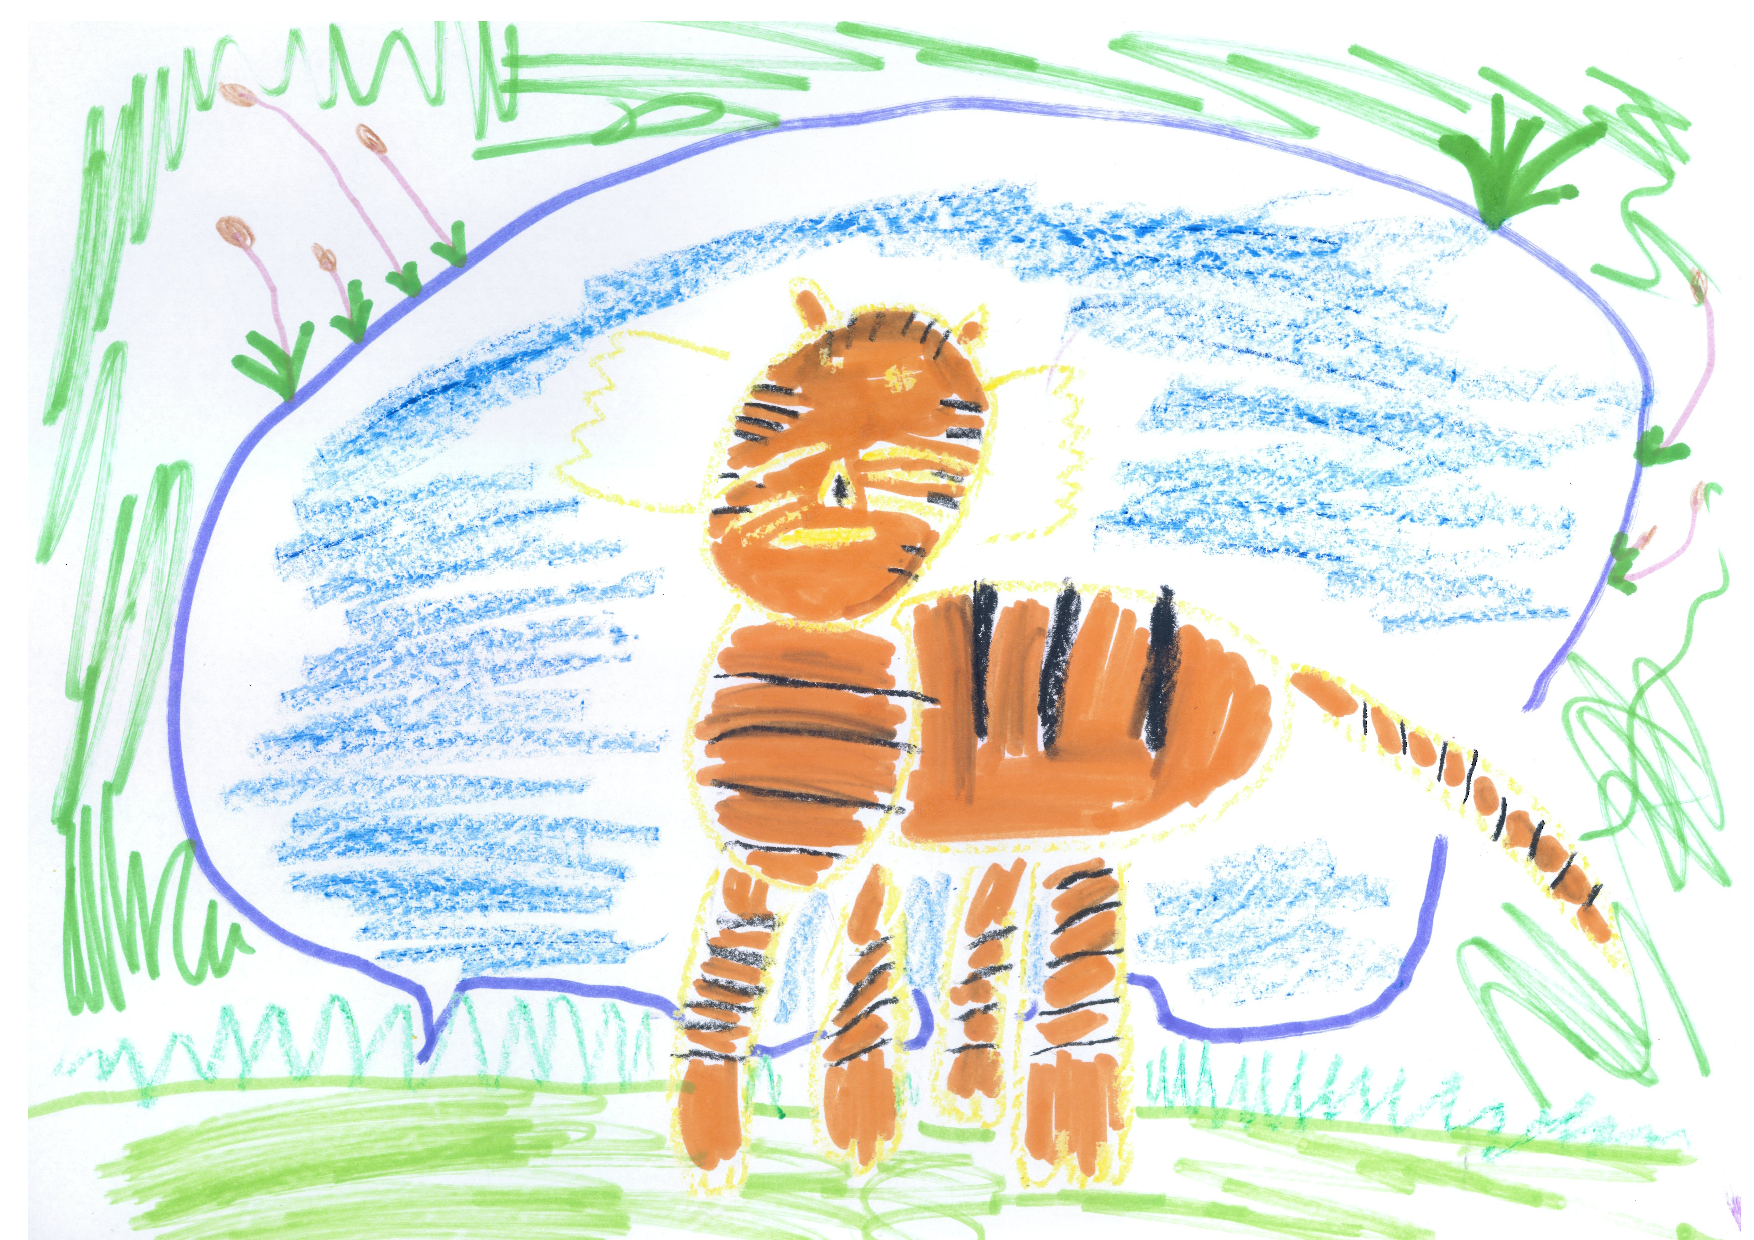
\includegraphics[width=\textwidth]{bilder/tiger.pdf}
    \end{figure}
    \clearpage
}


Aber Shirkan war wie verrückt. Er hat sich auf die Herde gestürzt. Eine Elephantenkuh mit einem Jungen ist es dann doch zu viel geworden. Sie hat den Tiger einfach mit dem Rüssel geschnappt und weit ins Dickicht geworfen. Shirkan war dann einige Tage nicht mehr zu sehen. So lange die Elephanten da waren, hat sich Shirkan nicht blicken lassen.

Die anderen Tiere sind erst zögerlich und dann in riesigen Scharen in den See gesprungen. Ein unglaublicher Anblick war das. Wenn Tiere eine Party feiern, dann sieht das wohl so aus. Da haben die unterschiedlichsten Tiere buchstäblich im Wasser miteinander gespielt. Der Dal Kar war für einige Tage fast nur noch Schaum von den vielen Tieren.

Aber nach circa einer Woche sind die Elephanten weiter gezogen. Und als sie weg waren, war Shirkan zurück. Ich hatte das Gefühl, noch grimmiger als vorher. Immer sprungbereit ist er vor dem Eingang zum See hin und her patrolliert und hat mit seinem Schwanz auf den Boden geschlagen.

Aber noch etwas ist passiert. Die Lust der Tiere, im See zu baden ist von den paar Tagen nicht kleiner geworden, sondern schien noch gewachsen zu sein. Auch sie sind immer forscher in Richtung See und damit auf Shirkan zu. Immer wieder haben es Wildschweine und Antilopen versucht, an Shirkan vorbei zu kommen. Hin rennen, ihn provozieren und schnell wieder weg. Immer wieder haben sie das gemacht, was Shirkan viel Kraft gekostet hat. 

Und plötzlich, am zweiten oder dritten Tag nach den Elephanten, war es plötzlich anders. Ein Büffel hat sein Glück versucht, ist aber auch wieder vertrieben worden. Aber an statt zurück in den Schutz des Dschungels zu fliehen, hat er sich plötzlich wieder umgedreht und den Kopf gesenkt und mit den Hufen gescharrt, als Zeichen, angreifen zu wollen. Plötzlich war es sehr viel stiller im Wald. Es war richtig spürbar, dass die anderen Tiere ihre Blicke nur auf die beiden gerichtet hatten. 

Natürlich ist ein Büffel eigentlich einem so grossen Tiger unterlegen, aber ich dachte, wenn Shirkan so erschöpft ist, hat der bulle vielleicht eine Chance. Und tatsächlich rennt er mit gesenkten Hörnern auf Shirkan los, der sich sprungbereit macht, um auf dessen Rücken springen zu können. Aber noch bevor der Bulle da ist, schiesst ein Wildschwein aus dem gebüsch und rammt Shirkan in die Seite. und gleich noch eins. Shirkan schlägt um sich, kann aber keines erwischen. Dann kommen Antilopen, springen über ihn und schlagen ihn von oben mit ihren Hufen. Sie scheinen von allen Seiten zu kommen, Shirkan weiss nicht, wo er als erstes hinschlagen soll. Von allen Seiten wird er bedrängt. 

Und dann kommt der grosse Aufschlag. Der Bulle rammt seine Hörner mit voller Wucht gegen Shirkan. Andere Bullen folgen. Shirkan ist zwar schwer getroffen, kann aber aufstehen. Und seitdem ich ihn kenne, macht er zum ersten Mal genau das richtige: er reisst aus. Schleppt sich ins Gebüsch und verschwindet. 

Ich bin dann noch einige Wochen dort geblieben, hab ihn aber nie mehr gesehen. Der See hat einige zeit von Tieren nur so gewimmelt, das hat sich aber schnell normalisiert. Der See gehört jetzt wieder allen Tieren, auch wenn hin und wieder Tiger vorbei kommen. Aber von denen ist einer länger als ein paar Tage geblieben.\hfill {\color{DeepPink}\decofourleft}
